%-----------------------------------------------------------------------
%
%     This file is part of the Code_Saturne Kernel, element of the
%     Code_Saturne CFD tool.
%
%     Copyright (C) 1998-2008 EDF S.A., France
%
%     contact: saturne-support@edf.fr
%
%     The Code_Saturne Kernel is free software; you can redistribute it
%     and/or modify it under the terms of the GNU General Public License
%     as published by the Free Software Foundation; either version 2 of
%     the License, or (at your option) any later version.
%
%     The Code_Saturne Kernel is distributed in the hope that it will be
%     useful, but WITHOUT ANY WARRANTY; without even the implied warranty
%     of MERCHANTABILITY or FITNESS FOR A PARTICULAR PURPOSE.  See the
%     GNU General Public License for more details.
%
%     You should have received a copy of the GNU General Public License
%     along with the Code_Saturne Kernel; if not, write to the
%     Free Software Foundation, Inc.,
%     51 Franklin St, Fifth Floor,
%     Boston, MA  02110-1301  USA
%
%-----------------------------------------------------------------------
%

\programme{inimas}

\vspace{1cm}
%%%%%%%%%%%%%%%%%%%%%%%%%%%%%%%%%%
%%%%%%%%%%%%%%%%%%%%%%%%%%%%%%%%%%
\section{Fonction}
%%%%%%%%%%%%%%%%%%%%%%%%%%%%%%%%%%
%%%%%%%%%%%%%%%%%%%%%%%%%%%%%%%%%%
Le but de ce sous-programme est principalement de calculer le flux de masse aux
faces. Il prend une variable vectorielle associ\'ee au centre des cellules
(g\'en\'eralement la vitesse), la projette aux faces en la multipliant par la
masse volumique, et la multiplie scalairement par le vecteur surface.
Plus g\'en\'eralement, \fort{inimas} est aussi appel\'e comme premi\`ere \'etape
du calcul d'une divergence (terme en $\dive(\rho\tens{R})$ en
$R_{ij}-\varepsilon$, filtre Rhie \& Chow, ...).

%%%%%%%%%%%%%%%%%%%%%%%%%%%%%%%%%%
%%%%%%%%%%%%%%%%%%%%%%%%%%%%%%%%%%
\section{Discr\'etisation}
%%%%%%%%%%%%%%%%%%%%%%%%%%%%%%%%%%
%%%%%%%%%%%%%%%%%%%%%%%%%%%%%%%%%%

La figure \ref{Base_Inimas_fig_geom} rappelle les diverses d\'efinitions g\'eom\'etriques
pour les faces internes et les faces de bord. On notera
$\displaystyle \alpha=\frac{\overline{FJ^\prime}}{\overline{I^\prime J^\prime}}$ (d\'efini aux faces
internes uniquement).

\begin{figure}[h]
\parbox{8cm}{%
\centerline{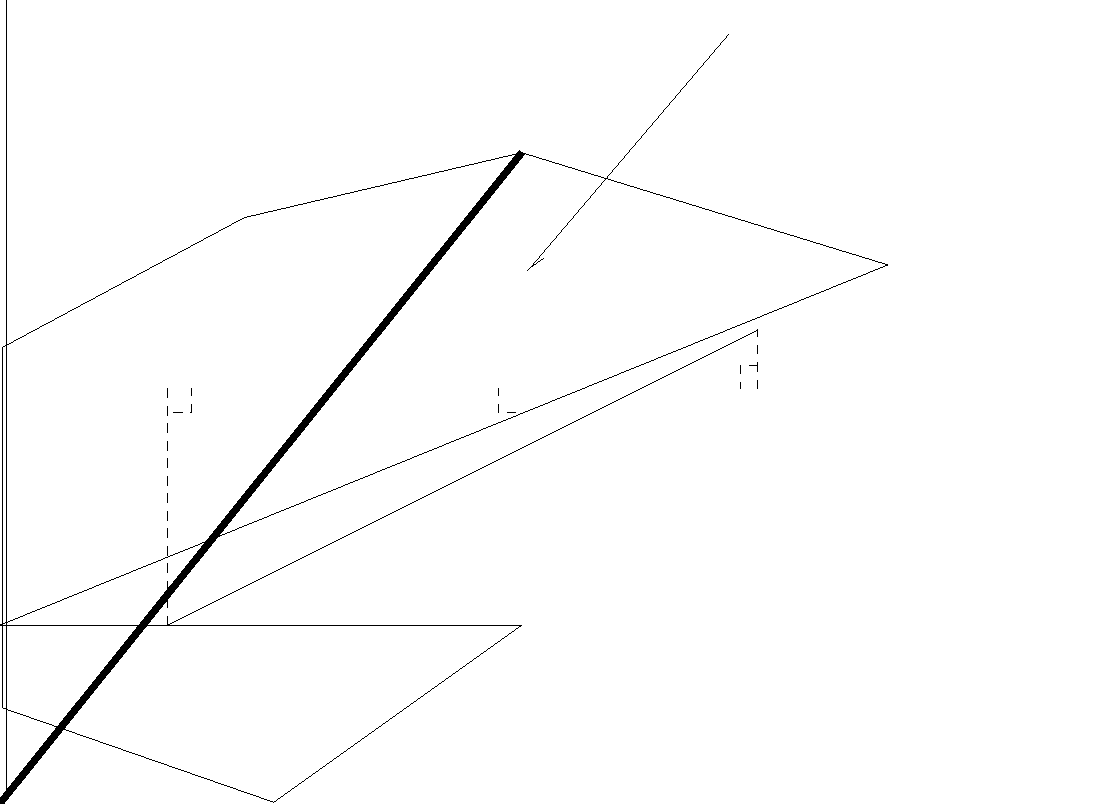
\includegraphics[height=4cm]{\repgraphics/facette}}}
\parbox{8cm}{%
\centerline{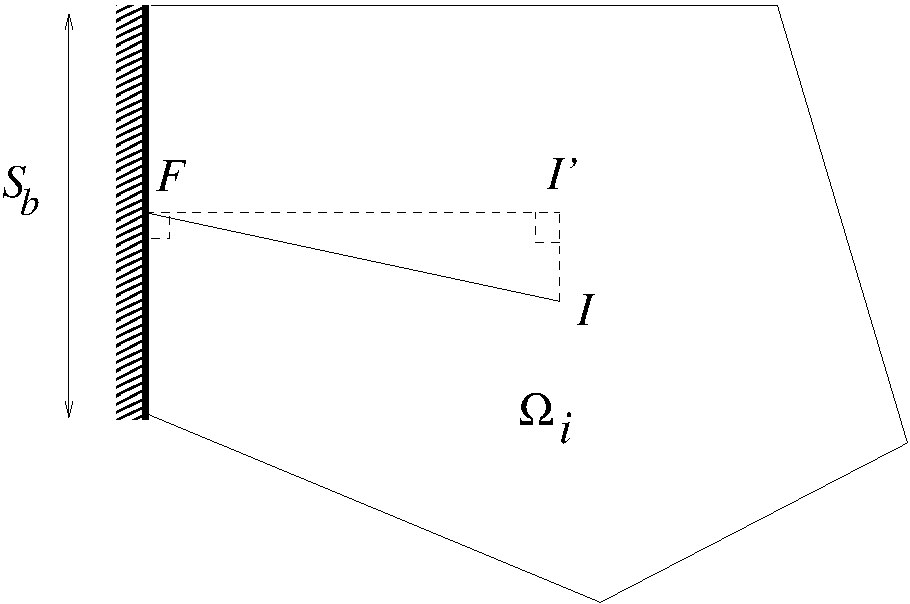
\includegraphics[height=4cm]{\repgraphics/facebord}}}
\caption{\label{Base_Inimas_fig_geom}D\'efinition des diff\'erentes entit\'es
g\'eom\'etriques pour les faces internes (gauche) et de bord (droite).}
\end{figure}


\subsection{Faces internes}
On ne conna\^\i t pas la masse volumique \`a la face, cette derni\`ere doit donc
aussi \^etre interpol\'ee. On utilise la discr\'etisation suivante :

\begin{equation}
(\rho \vect{u})_F = \alpha(\rho_I \vect{u}_I)
+(1-\alpha)(\rho_J \vect{u}_J)
+\ggrad\!(\rho\vect{u})_O.\vect{OF}
\end{equation}
La partie en $\alpha(\rho_I \vect{u}_I)
+(1-\alpha)(\rho_J \vect{u}_J)$ correspondant en fait \`a
$(\rho\vect{u})_O$. Le gradient en $O$ est calcul\'e par interpolation :
$\displaystyle\ggrad\!(\rho\vect{u})_O=
\frac{1}{2}\left[\ggrad\!(\rho\vect{u})_I+\ggrad\!(\rho\vect{u})_J\right]$. La
valeur $\displaystyle\frac{1}{2}$ s'est impos\'ee de mani\`ere heuristique au
fil des tests
comme apportant plus de stabilit\'e \`a l'algorithme global qu'une interpolation
faisant intervenir $\alpha$. L'erreur commise sur $\rho\vect{u}$ est en
$O(h^2)$.


\subsection{Faces de bord}
Le traitement des faces de bord est n\'ecessaire pour y calculer le flux de
masse, bien s\^ur, mais aussi pour obtenir des conditions aux limites pour le
calcul du $\ggrad\!(\rho \vect{u})$ utilis\'e pour les faces internes.

Pour les faces de bord, on conna\^\i t la valeur de $\rho_F$, qui est stock\'ee
dans la variable \var{ROMB}. De plus, les conditions aux limites pour $\vect{u}$
sont donn\'ees par des coefficients $A$ et $B$ tels que :
\begin{equation}
u_{k,F} = A_k + B_ku_{k,I^\prime} =
A_k + B_k\left(u_{k,I} + \grad\!(u_k)_I.\vect{II^\prime}\right)
\end{equation}
($k\in\{1,2,3\}$ est la composante de la vitesse, l'erreur est en $O(B_kh)$)

On a donc \`a l'ordre 1 :
\begin{equation}
(\rho u_k)_F = \rho_F\left[A_k + B_k\left(u_{k,I} +
\grad\!(u_k)_I.\vect{II^\prime}\right)\right]
\end{equation}

Mais pour utiliser cette formule, il faudrait calculer $\ggrad\!(\vect{u})$ (trois
appels \`a \fort{GRDCEL}), alors qu'on a d\'ej\`a calcul\'e
$\ggrad\!(\rho\vect{u})$ pour les faces internes. Le surco\^ut en temps serait alors
important. On r\'e\'ecrit donc :
\begin{eqnarray}
(\rho u_k)_F & = & \rho_F A_k + \rho_F B_ku_{k,I^\prime}\\
& = & \rho_F A_k + B_k\frac{\rho_F}{\rho_{I^\prime}}(\rho u_k)_{I^\prime}
\label{Base_Inimas_eq_rhoufacea}\\
& = & \rho_F A_k + B_k\frac{\rho_F}{\rho_{I^\prime}}(\rho u_k)_I
+B_k\frac{\rho_F}{\rho_{I^\prime}}\grad\!(\rho u_k)_I.\vect{II^\prime}
\label{Base_Inimas_eq_rhoufaceb}
\end{eqnarray}

Pour calculer les gradients de $\rho\vect{u}$, il faudrait donc en th\'eorie
utiliser les coefficients de conditions aux limites \'equivalents :\\
$\tilde{A}_k = \rho_F A_k$\\
$\displaystyle \tilde{B}_k = B_k\frac{\rho_F}{\rho_{I^\prime}}$

Ceci para\^\i t d\'elicat, \`a cause du terme en
$\displaystyle \frac{\rho_F}{\rho_{I^\prime}}$, et en particulier \`a l'erreur
que l'on peut commettre sur $\rho_{I^\prime}$ si la reconstruction des gradients
est imparfaite (sur des maillages fortement non orthogonaux par exemple).
On r\'e\'ecrit donc l'\'equation
(\ref{Base_Inimas_eq_rhoufaceb}) sous la forme suivante :
\begin{equation}
(\rho u_k)_F=\rho_F A_k + B_k\frac{\rho_I\rho_F}{\rho_{I^\prime}}u_{k,I}
+B_k\frac{\rho_F}{\rho_{I^\prime}}\grad\!(\rho u_k)_I.\vect{II^\prime}
\end{equation}


Pour le calcul du flux de masse au bord, on va faire deux approximations. Pour
le deuxi\`eme terme, on va supposer $\rho_{I^\prime}\approx\rho_I$ (ce qui
conduit \`a une erreur en $O(B_kh)$ sur $\rho\vect{u}$ si
$\rho_{I^\prime}\ne \rho_I$). Pour le
troisi\`eme terme, on va supposer $\rho_{I^\prime}\approx\rho_F$. Cette
derni\`ere approximation est plus forte, mais elle n'intervient que dans la
reconstruction des non-orthogonalit\'es ; l'erreur finale reste donc faible
(erreur en $O(B_kh^2)$ sur $\rho\vect{u}$ si
$\rho_{I^\prime}\ne \rho_F$).
Et au final, le flux de masse au bord est calcul\'e par :
\begin{equation}
\dot{m}_F = \sum\limits_{k=1}^{3}\left[\rho_F A_k + B_k\rho_Fu_{k,I}
+B_k\grad\!(\rho u_k)_I.\vect{II^\prime}\right]S_k
\end{equation}

Pour le calcul des gradients, on repart de l'\'equation (\ref{Base_Inimas_eq_rhoufacea}), sur
laquelle on fait l'hypoth\`ese que $\rho_{I^\prime}\approx\rho_F$. Encore une
fois, cette hypoth\`ese peut \^etre assez forte, mais les gradients obtenus ne
sont utilis\'es que pour des reconstructions de non-orthogonalit\'es ; l'erreur
finale reste donc l\`a encore assez faible.
Au final, les gradients sont calcul\'es \`a partir de la formule suivante :
\begin{equation}
(\rho u_k)_F = \rho_F A_k + B_k(\rho u_k)_{I^\prime}
\end{equation}
ce qui revient \`a utiliser les conditions aux limites suivantes pour
$\rho \vect{u}$:\\
$\tilde{A}_k = \rho_F A_k$\\
$\tilde{B}_k = B_k$

\minititre{Remarque}

Dans la plupart des cas, les approximations effectu\'ees n'engendrent aucune
erreur. En effet :\\
- dans le cas d'une entr\'ee on a g\'en\'eralement $B_k=0$, avec un flux de
masse impos� par la condition � la limite.\\
- dans le cas d'une sortie, on a g\'en\'eralement flux nul sur les scalaires
donc sur $\rho$, soit \mbox{$\rho_F=\rho_{I^\prime}=\rho_I$}.\\
- dans le cas d'une paroi, on a g\'en\'eralement $B_k=0$ et le flux de masse
est impos� nul.\\
- dans le cas d'une sym\'etrie, on a g\'en\'eralement
$\rho_F=\rho_{I^\prime}=\rho_I$ et le flux de masse est impos� nul.\\
Pour sentir un effet de ces approximations, il faudrait par exemple une paroi
glissante ($B_k\ne0$) avec un gradient de temp\'erature ($\rho_F\ne\rho_I$).

%%%%%%%%%%%%%%%%%%%%%%%%%%%%%%%%%%
%%%%%%%%%%%%%%%%%%%%%%%%%%%%%%%%%%
\section{Mise en \oe uvre}
%%%%%%%%%%%%%%%%%%%%%%%%%%%%%%%%%%
%%%%%%%%%%%%%%%%%%%%%%%%%%%%%%%%%%

La vitesse est pass\'ee par les arguments \var{UX}, \var{UY} et \var{UZ}. Les
conditions aux limites de la vitesse sont \var{COEFAX}, \var{COEFBX}, ... Le
flux de masse r\'esultat est stock\'e dans les variables \var{FLUMAS} (faces
internes) et \var{FLUMAB} (faces de bord). \var{QDMX}, \var{QDMY} et \var{QDMZ}
sont des variables de travail qui serviront \`a stocker $\rho\vect{u}$, et
\var{COEFQA} servira \`a stocker les $\tilde{A}$.

\etape{Initialisation \'eventuelle du flux de masse}
Si \var{INIT} vaut 1, le flux de masse est remis \`a z\'ero. Sinon, le
sous-programme rajoute aux variables \var{FLUMAS} et \var{FLUMAB} existantes le
flux de masse calcul\'e.


\etape{Remplissage des tableaux de travail}
$\rho\vect{u}$ est stock\'e dans \var{QDM}, et $\tilde{A}$ dans \var{COEFQA}.


\etape{Cas sans reconstruction}
On calcule alors directement\\
$\displaystyle \var{FLUMAS}=\sum\limits_{k=1}^{3}\left[
\alpha(\rho_I u_{k,I})+(1-\alpha)(\rho_J u_{k,J})\right]S_k$\\
et\\
$\displaystyle \var{FLUMAB}=\sum\limits_{k=1}^{3}\left[
\rho_F A_k + B_k\rho_Fu_{k,I}\right]S_k$


\etape{Cas avec reconstruction}
On r\'ep\`ete trois fois de suite les op\'erations suivantes, pour $k=1$, 2 et 3
:\\
- Appel de \fort{GRDCEL} pour le calcul de $\grad\!(\rho u_k)$.\\
- Mise \`a jour du flux de masse\\
$\displaystyle \var{FLUMAS}=\var{FLUMAS} + \left[
\alpha(\rho_I u_{k,I})+(1-\alpha)(\rho_J u_{k,J})
+\frac{1}{2}\left[\grad\!(\rho u_k)_I+\grad\!(\rho u_k)_J\right]
.\vect{OF}\right]S_k$\\
et\\
$\displaystyle \var{FLUMAB}=\var{FLUMAB}+\left[
\rho_F A_k + B_k\rho_Fu_{k,I}
+B_k\grad\!(\rho u_k)_I.\vect{II^\prime}\right]S_k$


\etape{Annulation du flux de masse au bord}
Quand le sous-programme a \'et\'e appel\'e avec la valeur \var{IFLMB0=1}
(c'est-\`a-dire quand il est r\'eellement appel\'e pour calculer un flux de
masse, et pas pour calculer le terme en $\dive(\rho\tens{R})$ par exemple), le flux
de masse au bord \var{FLUMAB} est forc\'e \`a 0, pour les faces de paroi et de
sym\'etrie (identifi\'ees par \var{ISYMPA=0}).
